\documentclass[a4paper, 12pt]{report}
\usepackage[a4paper,hmargin={3cm,2.5cm},vmargin={2.5cm,2.5cm}]{geometry}
\usepackage{amsfonts} % if you want blackboard bold symbols e.g. for real numbers
\usepackage{graphicx} % if you want to include jpeg or pdf pictures
\usepackage[english]{babel}
\usepackage[autostyle, english = american]{csquotes}
\usepackage{multicol}
\usepackage{lipsum}
\usepackage{subfig}
\usepackage{float}
\usepackage{blindtext}
\usepackage{fancyhdr}
\pagestyle{fancy}
\lhead{}
\rhead{Unit Converter}
\usepackage{tikz}
\usetikzlibrary{calc}
\usepackage{eso-pic}
\usepackage{lipsum}



\begin{document}



%========================================================= %
%================begin of title page====================== %
% The frontmatter environment for everything that comes with roman numbering\
%============================================= %
\newenvironment{frontmatter}{}{}
\begin{frontmatter}
%%%%%%%%%%%%%%%%%%%%%%%%%%%%%%%%%%%%%%%%%%%%%%%%%%%%%%%%%%%%%%%%%%%
\begin{titlepage}
%\AddToShipoutPictureBG
\begin{center}
\textup{\large  \textbf{Savitribai Phule Pune University}\\\textbf{Modern Education Society’s College of Engineering, Pune}}\\19, Bund Garden, V.K. Joag Path, Pune – 411001.\\[0.5cm]\textbf{ACCREDITED BY NAAC WITH \enquote{A} GRADE (CGPA – 3.13)}\\[0.5cm]\textbf{\large DEPARTMENT OF COMPUTER ENGINEERING}
\begin{center}
\begin{figure}[h]
\centering

\includegraphics[width=0.3\linewidth]{./logo}
\end{figure}
\end{center}
\textup{\large  A MINI PROJECT REPORT\\[0.8cm]ON}\\[0.8cm]
\begin{LARGE}
{\textbf {\enquote{UNIT CONVERTER}}}\end{LARGE}\\[1.2cm]
\begin{large}\textbf {T.E. (COMPUTER)}
\end{large}\\[1cm]
\textit{SUBMITTED BY}\\[0.5cm]
\begin{large}\textbf{Mr. Aditya Ujeniya}\hspace{1.4cm}
\textbf{Roll No:  70}\\\end{large}
\begin{large}\textbf{Mr. Dheeraj  Thambare}\hspace{0.5cm}
\textbf{Roll No: 68}\\\end{large}
\begin{large}\textbf{Mr. Shubham Shingade}\hspace{0.5cm}
\textbf{Roll No: 65}\\[1cm]\end{large}
\textit{UNDER THE GUIDANCE OF}\\[0.7cm]
\begin{large}\textbf{PROF. S. S. RASKAR}\\[0.3cm]\end{large}
\textbf{(Academic Year: 2017-2018)}

\vfill
\end{center}
\end{titlepage}
%================begin of certificate page======================

\begin{titlepage}
\begin{tikzpicture}[overlay,remember picture]
\draw[line width=4pt]
    ($ (current page.north west) + (1cm,-1cm) $)
    rectangle
    ($ (current page.south east) + (-1cm,1cm) $);
\draw[line width=1.5pt]
    ($ (current page.north west) + (1.2cm,-1.2cm) $)
    rectangle
    ($ (current page.south east) + (-1.2cm,1.2cm) $);
\end{tikzpicture}
\begin{center}
\textup{\large  \textbf{Savitribai Phule Pune University}\\\textbf{Modern Education Society’s College of Engineering, Pune}}\\19, Bund Garden, V.K. Joag Path, Pune – 411001.\\[0.8cm]\textbf{ACCREDITED BY NAAC WITH \enquote{A} GRADE (CGPA – 3.13)}\\[0.8cm]\textbf{\large DEPARTMENT OF COMPUTER ENGINEERING}

\begin{figure}[h]
\centering

\includegraphics[width=0.3\linewidth]{./logo}
\end{figure}
\begin{LARGE}
\textbf{\textit {Certificate}}\end{LARGE}\\[1.2cm]
This is to certify that mini project entitled\\[0.5cm]\large\textbf{\enquote{UNIT CONVERTER}}
\end{center}  
has been completed by Mr. Aditya Ujeniya( Roll No. 70 ) of TE COMP II in the Semester - II of academic year 2017-2018 in partial fulfillment of the Third Year of Bachelor degree in "Computer Engineering" as prescribed by the Savitribai Phule Pune University.
\vspace{3cm}
\begin{multicols}{2}
\begin{center}
\textbf{Prof S. S. Raskar\\Mini-project Guide}\hspace{5cm}\\
\end{center}
\begin{center}
\textbf{(Dr.(Mrs.) N. F. Shaikh)\\H.O.D}\\
\end{center}
\end{multicols}\vspace{0.6cm}
Place: MESCOE, Pune.\\
\hspace{0.5cm}Date:   /   /2017
\vfill

\end{titlepage}
%================end of title page======================
\pagenumbering{gobble}

\pagebreak

\newpage
\begin{center}
{\Large{\bf{\textit{ACKNOWLEDGEMENT}}\\[2cm]}}
\end{center}
\par \textit{It gives me great pleasure and satisfaction in presenting this mini project on “Unit Converter".} \\
\par \textit{I am thankful to and fortunate enough to get constant encouragement, support and guidance from all Teaching staffs of [Computer Dept] which helped us in successfully completing our project work. Also, I would like to extend our sincere esteems to all staff in laboratory for their timely support.} \\

\par \textit{I have furthermore to thank Computer Department HOD}  {\bf Dr.(Mrs.) N. F. Shaikh} \textit{and} {\bf Prof. S. S. Raskar} \textit{to encourage me to go ahead and for continuous guidance. I also want to thank {\bf Prof. S. H. Pisey} for all her assistance and guidance for preparing report.}\\
\par \textit{I would like to thank all those, who have directly or indirectly helped me for the completion of the work during this mini project.}
\vspace{0.8in}
\begin{flushright}
{Aditya Ujeniya}\\
\hspace*{0.1in}{T.E. Computer}\\
\hspace*{0.1in}{Roll no. : 70}\\
\end{flushright}
\pagenumbering{roman}
\setcounter{page}{1}
\newpage
\tableofcontents
\listoffigures
\renewcommand{\footrulewidth}{1pt}
\lfoot{Modern Education Society’s College of Engineering}
%%%%%%%%%%%%%%% Abstract %%%%%%%%%%
%\newpage
\begin{abstract}
\par This project is based on a Android application which helps user for unit conversion called as Unit Converter. The application is helpful, accurate and fast enough to fulfill the user’s requirements. The application works fluently on offline mode and provides various units categories for conversion.\\
\par It’s a Android based application developed in Android Studio IDE with the use of Fragments, SQLite Database and a simple Navigation Drawer. The application is highly compatible with variety of API Levels above API 20 (Lolipop). The main aim of application is to provide offline support with a simple interface for conversion of units.It consist of US(Metric) and UK(Imperial) units as well.
\\\\
\hspace*{0.8cm}The beautiful Material Design user interface allows for quick and easy conversions from a number in one unit to another. The goal is to keep it simple - you won't be overwhelmed with an excess of options and settings, allowing you to perform your desired conversion as quickly as possible. Perfect for work, school or in the kitchen.
\vspace{0.3cm}
\end{abstract}
%================================================ %
% The frontmatter environment for everything that comes with roman numbering %
\end{frontmatter}
%%%%%%%%%%%%%%%%%%%%%%%%%%%%%%%%%%%%%%%

\newpage
\pagenumbering{arabic}
%%%%%%%%% MAIN TEXT STARTS HERE %%%%%%%%%%
\chapter{INTRODUCTION}\hspace{0.8cm}Unit converter is used to convert values. It is a basic converter that converts values from one unit to the other unit. For example, if we want to convert any factor using a predefined ratio, then we have to mulitply that factor by the user specified value. Hence, each and every Unit is having its own factor.
\newline\\
\hspace*{0.8cm}
The described conversion factors act as fractions equaling 1. When conversion factors are used to convert units, we will multiply the user muliplier factor by the conversion factor to get the same measurements expressed in new units. There is consistent need to maintain correct values, to provide accurate measurements that will be used on a professional level. 
\section{Introduction}
What is a unit ?\\\\
\hspace*{0.8cm}Standard unit or system of units by mean of which a quantity is accounted for and expressed
Definitive or determinate quantity adopted as a standard of measurement and exchange. \\\\
\hspace*{0.8cm}A quantity generally accepted as a standard for exchange.
Available unit conversions include:\\
\\-     Temperature (celsius, fahrenheit, kelvin, etc)\\
-     Length (kilometer, miles, meter, yard, feet, etc)\\
-     Mass/Weight (kilogram, pound, ounce, ton, stone, etc)\\
-     Speed (km/h, mph, knot, etc)\\
-     Area (square kilometer, square mile, hectare, acre, etc)\\
-     Cooking Volume (teaspoon, tablespoon, cup, pint, quart, ounce, etc)\\
-     Pressure (kilopascal, bar, PSI, etc)\\
-     Power (watt, kilowatt, horsepower, etc)\\
-     Energy (joule, calorie, BTU, etc)\\
-     Fuel Consumption (miles per gallon, liters per 100km, etc)\\
-     Digital Storage (bit, byte, megabytes, gigabytes, etc)\\

\section{Motivation}
\hspace{0.8cm}
In todays era,whichever field a person is working in, needs to analyze and convert the various contents including units. A person working in Civil field needs length conversions, a person working in Mechanical field needs speed, energy, power conversion, a person working in Software field needs digital storage conversion and so on. \\\\
\hspace*{0.8cm}There is tremendous need for metric as well as imperial units conversion. So we have developed the android application, in offline mode, such that it will cover all of the needed units for conversion. The ON-THE-GO offline portability is the application's quality which allows user to use if whenever and whereever required.
\chapter{PROBLEM  STATEMENT}
\section{Problem Statement}
\hspace{0.8cm}A portable Android application that provides various conversion units category wise with a simple interface and offline facility. Accuracy should be maintained while providing various units. The ambuiguity between units of ToUnits and FromUnits should be reduced. The categorized units should be able to provide organized and simple interface.\\
\section{Explanation}
\hspace{0.8cm}UnitConverter allows user to choose from variety of unit conversion categories.  Offline avaliablity and accurate results are the speciality of the applications. Various units are avaliable that are used on daily basis as well as on professional level. The categorized units allow easy searchingg of a specific unit.
\chapter{SOFTWARE REQUIREMENT SPECIFICATION}
\section{Software and Hardware Requirement}
\subsection{Software Requirements}
\begin{itemize}
\item Android Studio 2.3.3
\item Android SDK 24+
\item API Level 20+ (Lolipop) on Android Device
\item SQLite database
\end{itemize}
\subsection{Hardware Requirements}
\begin{itemize}
\item Dual Core Processor
\item Min 10Mb Ram
\item Min 10Mb of storage space
\end{itemize}
\section{ER Diagram}
\begin{center}
\begin{figure}[h]
\centering
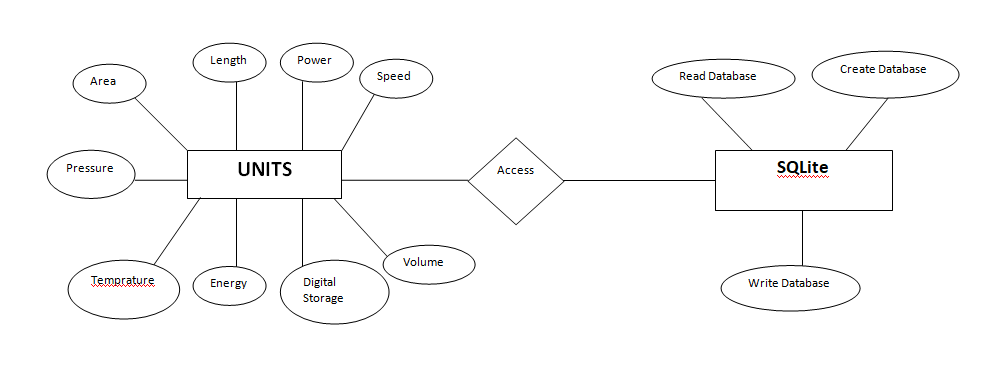
\includegraphics[scale = 0.5]{./er}
\caption{SQLite to Fragments ER Diagram}
\end{figure}
\end{center}
\section{Database Connectivity}
\subsection{SQLite Database}
\hspace{0.8cm}SQLite is a relational database management system contained in a C programming library. In contrast to many other database management systems, SQLite is not a client–server database engine. Rather, it is embedded into the end program.
\\\hspace*{0.8cm}
SQLite is ACID-compliant and implements most of the SQL standard, using a dynamically and weakly typed SQL syntax that does not guarantee the domain integrity.
\\\hspace*{0.8cm}
SQLite is a popular choice as embedded database software for local/client storage in application software such as web browsers. It is arguably the most widely deployed database engine, as it is used today by several widespread browsers, operating systems, and embedded systems (such as mobile phones), among others.SQLite has bindings to many programming languages.
\subsection{Usage}
\hspace{0.8cm}UnitConverter is maintaing a class called UnitDBHelper that contains the methods to access the database contents. It helps in creating, writing and reading the database.\\\\
\hspace*{0.8cm}Just by using the given syntax, it will initialize the SQLite database and will be able to read as well as write into that database.\\
\\\hspace*{1.5cm}\textbf{UnitDBHelper unitdbhelper = new UnitDBHelper();}\\\\
\hspace*{0.8cm}\textbf{unitdbhelper.getDatabase();} will return the cursor whhich will point to the starting entry of a table it is referencing to. Using the cursor, we can retrive each and every entry of the table.\\
\\\hspace*{0.8cm} It also allows retriving the specific value for desired unit. Just as we are requiring a specific unit value, it will roll over the entries of table and will return the specific \textbf{unit value}.

\chapter{IMPLEMENTATION OF PROJECT}
\section{Modules description}
\subsection{Activity}
\hspace{0.8cm}If you have worked with C, C++ or Java programming language then you must have seen that your program starts from main() function. Very similar way, Android system initiates its program with in an Activity starting with a call on onCreate() callback method. There is a sequence of callback methods that start up an activity and a sequence of callback methods that tear down an activity.
\\\hspace*{0.8cm}Given are the various lifecycle methods of Activity : 
\begin{enumerate}
\item onCreate() - This is the first callback and called when the activity is first created.
\item onStart() - This callback is called when the activity becomes visible to the user.
\item onResume() - This is called when the user starts interacting with the application.
\item onPause() - The paused activity does not receive user input and cannot execute any code and called when the current activity is being paused and the previous activity is being resumed.
\item onStop() - This callback is called when the activity is no longer visible.
\item onDestroy() - This callback is called before the activity is destroyed by the system.
\item onRestart() - This callback is called when the activity restarts after stopping it.
\end{enumerate}
\subsection{Fragment}
\hspace{0.8cm}This callback is called when the activity restarts after stopping it.A fragment has its own layout and its own behaviour with its own life cycle callbacks. You can add or remove fragments in an activity while the activity is running. You can combine multiple fragments in a single activity to build a multi-pane UI.\\\\
\hspace*{0.8cm}A fragment can be used in multiple activities. Fragment life cycle is closely related to the life cycle of its host activity which means when the activity is paused, all the fragments available in the activity will also be stopped. A fragment can implement a behaviour that has no user interface component.
\subsection{NavigationDrawer}
\hspace{0.8cm}The navigation drawer is a panel that displays the app’s main navigation options on the left edge of the screen. It is hidden most of the time, but is revealed when the user swipes a finger from the left edge of the screen or, while at the top level of the app, the user touches the app icon in the action bar.
\subsection{Java}
\hspace*{0.8cm}Java is a general-purpose computer programming language that is concurrent, class-based, object-oriented, and specifically designed to have as few implementation dependencies as possible. It is intended to let application developers "write once, run anywhere" (WORA), meaning that compiled Java code can run on all platforms that support Java without the need for recompilation. Java applications are typically compiled to bytecode that can run on any Java virtual machine (JVM) regardless of computer architecture. As of 2016, Java is one of the most popular programming languages in use, particularly for client-server web applications, with a reported 9 million developers. Java was originally developed by James Gosling at Sun Microsystems (which has since been acquired by Oracle Corporation) and released in 1995 as a core component of Sun Microsystems' Java platform. The language derives much of its syntax from C and C++, but it has fewer low-level facilities than either of them.\\\\
\hspace*{0.8cm}
The original and reference implementation Java compilers, virtual machines, and class libraries were originally released by Sun under proprietary licenses. As of May 2007, in compliance with the specifications of the Java Community Process, Sun relicensed most of its Java technologies under the GNU General Public License. Others have also developed alternative implementations of these Sun technologies, such as the GNU Compiler for Java (bytecode compiler), GNU Classpath (standard libraries), and IcedTea-Web (browser plugin for applets).\\\\
\hspace*{0.8cm}
The latest version is Java 9, released on September 21, 2017, and is one of the two versions currently supported for free by Oracle. Versions earlier than Java 8 are supported both by Oracle and other companies on a commercial basis.
\subsection{XML}
In computing, Extensible Markup Language (XML) is a markup language that defines a set of rules for encoding documents in a format that is both human-readable and machine-readable. The W3C's XML 1.0 Specification and several other related specifications—all of them free open standards—define XML.
\\\\\hspace*{0.8cm}
The design goals of XML emphasize simplicity, generality, and usability across the Internet. It is a textual data format with strong support via Unicode for different human languages. Although the design of XML focuses on documents, the language is widely used for the representation of arbitrary data structures such as those used in web services.
\newpage
\section{Screen shots of Project}
\begin{center}
\begin{figure}[h]
\centering
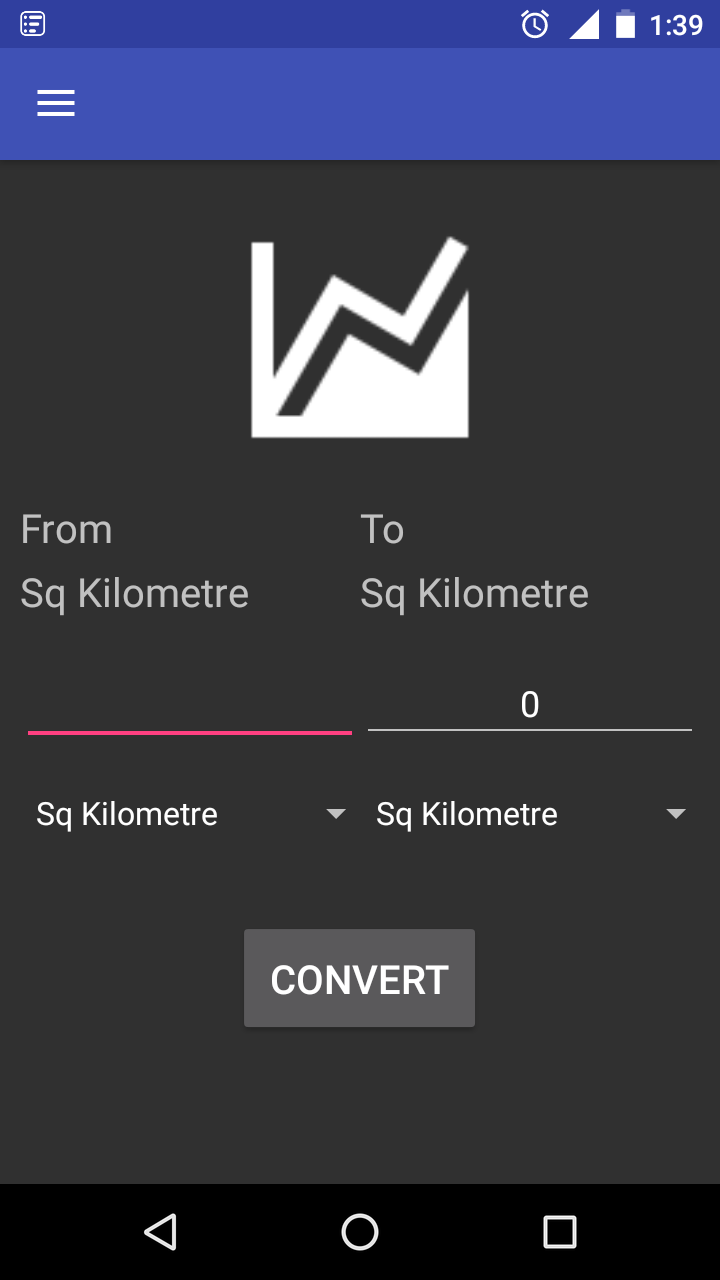
\includegraphics[scale = 0.35]{./ss1}
\caption{Introduction page and layout of conversion frame}
\end{figure}
\end{center}
\begin{center}
\begin{figure}
\centering
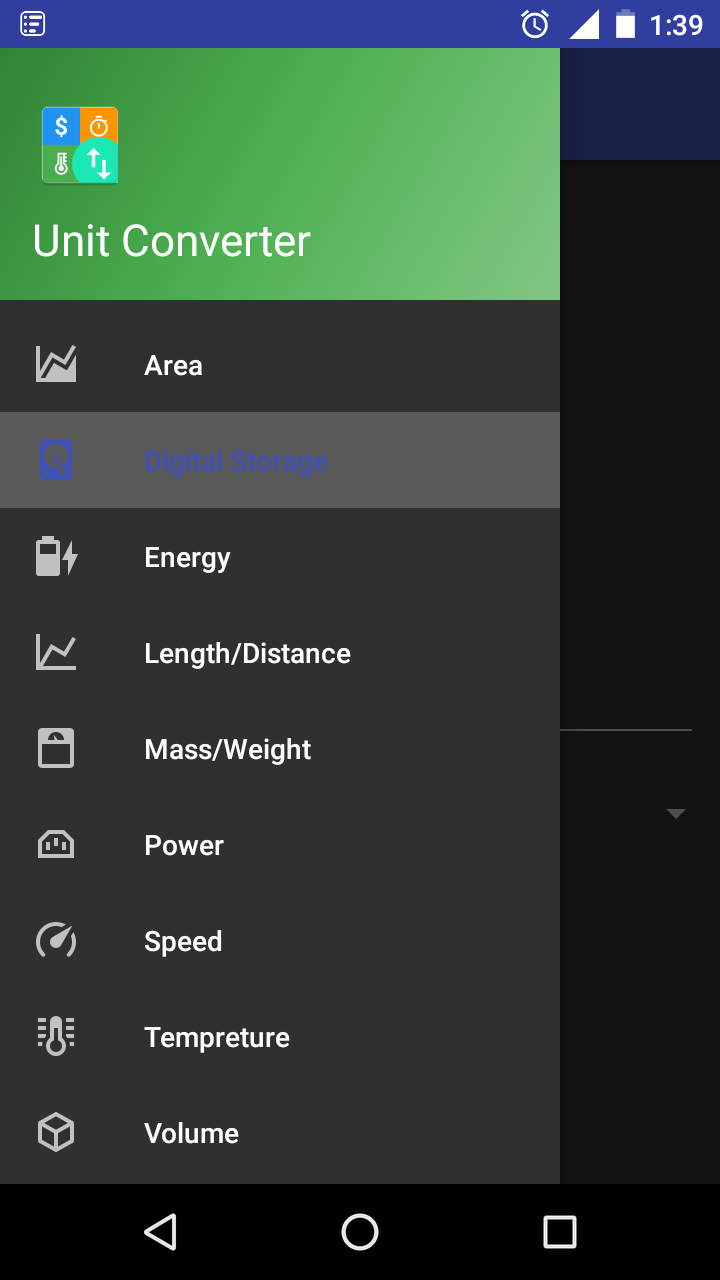
\includegraphics[scale = 0.35]{./ss2}
\caption{Navigation drawer containing various unit categories}
\end{figure}
\end{center}
\begin{center}
\begin{figure}
\centering
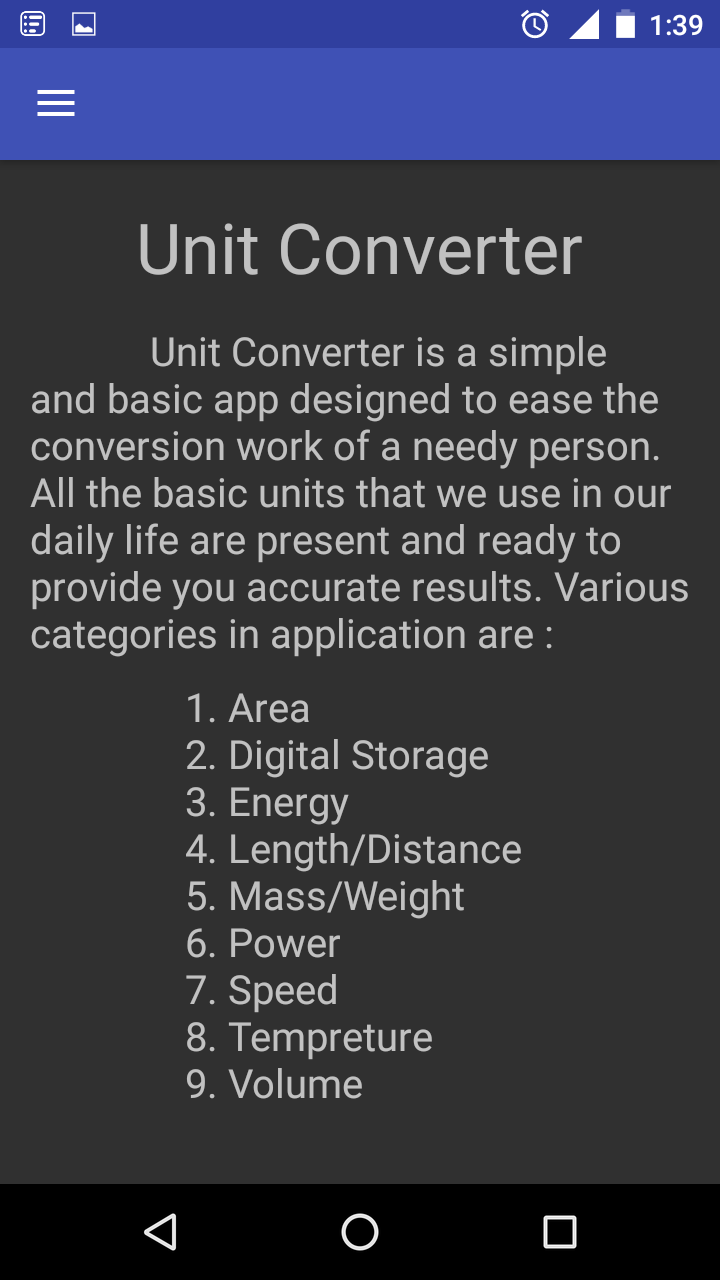
\includegraphics[scale = 0.35]{./ss3}
\caption{About Application}
\end{figure}
\end{center}
\begin{center}
\begin{figure}
\centering
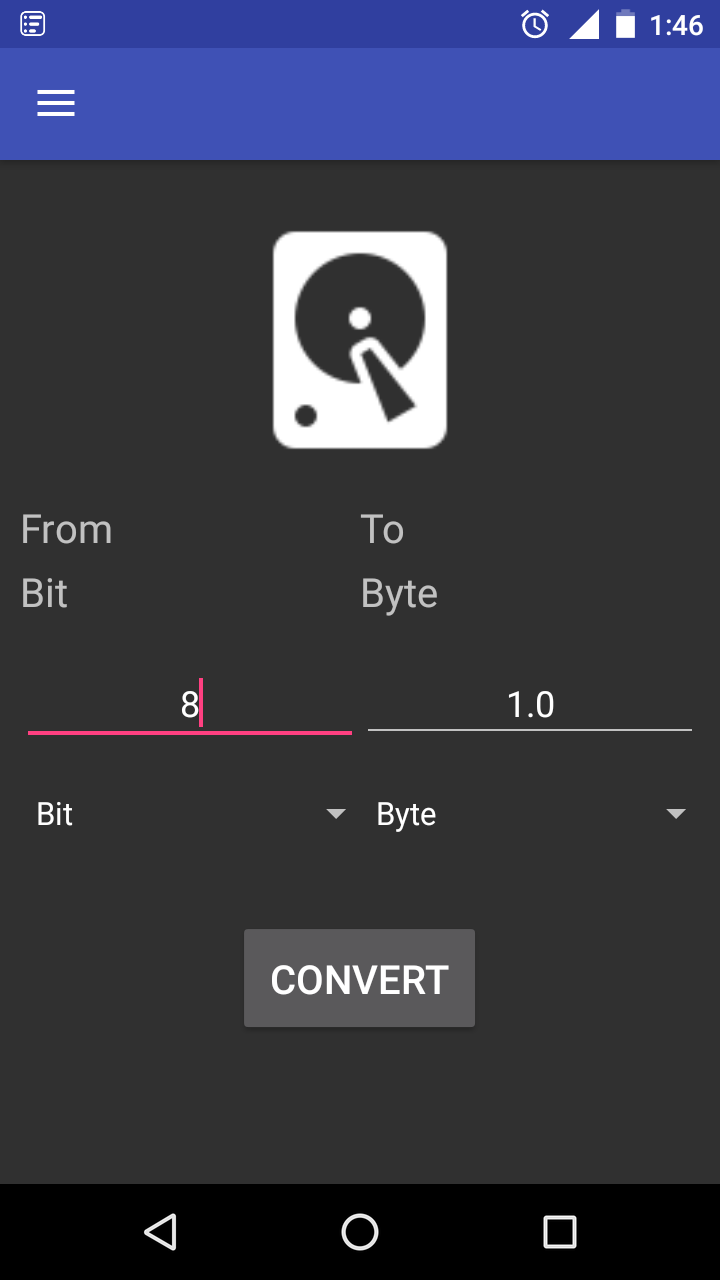
\includegraphics[scale = 0.35]{./ss4}
\caption{A sample converted value}
\end{figure}
\end{center}

\chapter{CONCLUSION}
\hspace{0.8cm}\textbf{This project taught us various rigorous excersizes that helped in developing the essential skillsets needed in industry. The main objective of offline portability using Android was achieved in the project as per requirement. Using SQLite database, the work was easily managed of storing the values and retriving them.\\\\\hspace*{0.8cm}Learnt various units used on daily basis as well at professional level. Various imperial and metric units also played important role to decide the future scope of the project. Working with team was encouragement as well as enjoyment.}
\end{document} 

